\chapter{Systemdesign}\label{Systemdesign}

\section{Pakkediagram}
Der er på baggrund af softwarearkitekturen lavet et pakkediagram, som kan ses på nedenstående Figur \ref{Pakkediagram}. Pakkediagrammet er en opdeling af systemets klasser i forskellige packages. I dette projekt er der valgt tre pakker. 

AutoSocograophyWPF inderholder alt, der hører til Grafisk brugergrænseflade (GUI), herunder de tre menuer, 3DscanMenu, StartMenu og UltrasoundMenu. 

ComputerVisionLibrary indeholder klasser, der har at gøre med 3D billedet og konvetering til et mesh, herunder ComputerVisionMaster, KinectsFusionizer og PLYExporter. 

RoboLibray pakken indeholder klasser som robotarmen skal benytte for at kunne flytte sig, herunder Analyzer, Data, Logic, Modbus, PathCreator, PathFeeder, Reader, RoboMaster, URPose og Writer. 

\begin{figure}[H]
    \centering
    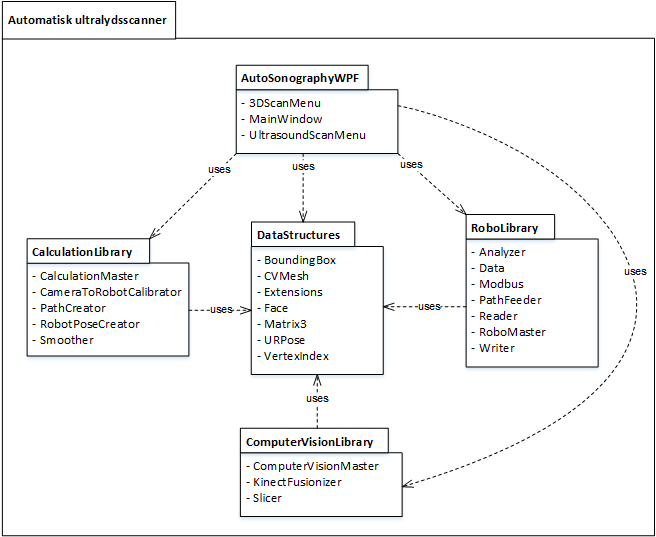
\includegraphics[width=0.5\textwidth]{figurer/d/Design/Pakkediagram}
    \caption{Pakkediagram for Automatisk Ultralydsscanner}
    \label{Pakkediagram}
\end{figure}
\newpage
\section{Klassediagram}
Dette afsnit beskriver klasserne fra pakkediagrammet. Klassediagrammerne viser strukturen i systemet og deres relationer. Hver klasse indeholder de vigtigste metoder og attributer i klassen, der udgør funktionaliteten i System. 

\subsection{GUI}
Skriv tekst her...

\begin{figure}[H]
    \centering
    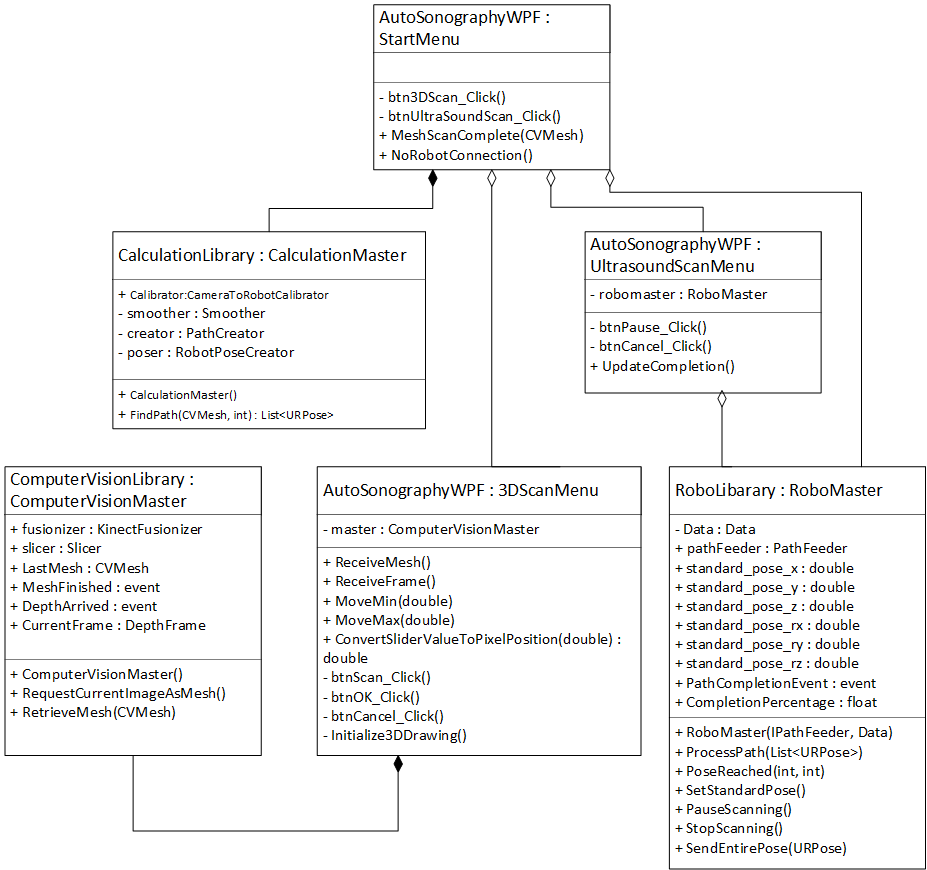
\includegraphics[width=1\textwidth]{figurer/d/Design/Class/uml_class_gui}
    \caption{KLassediagram for GUI}
    \label{class_gui}
\end{figure}
\newpage
\subsection{ComputerVisionLibrary}
Formålet med dette bibliotek er at få en afgrænset 3D scanning fra et 3D kamera.

KinectFusionizeren har til ansvar at åbne Kinect-sensoren, tage det nuværende dybdebillede fra sensoren og konvertere det til en mesh.

ComputerVisionMaster virker som den logiske grænseflade til KinectFusionizeren, hvor instansen af den nuværende mesh lagres her. Andre klasser kan subscribe til ComputerVisionMasteren for at høre hvornår der er en ny mesh tilgængelig.

\begin{figure}[H]
    \centering
    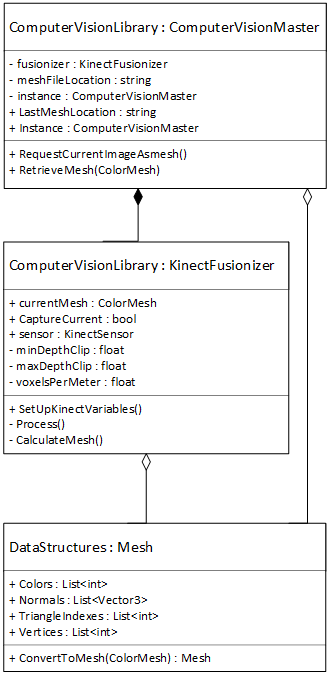
\includegraphics[width=0.5\textwidth]{figurer/d/Design/Class/uml_class_computervisionlibrary}
    \caption{KLassediagram for ComputerVisionLibrary}
    \label{class_ComputerVisionLib}
\end{figure}
\newpage
\subsection{ConversionLibrary}
Dette bibliotek agerer som bindeledet mellem ComputerVisionLibrary og RoboLibrary.
CameraToRobotCalibrator sørger for at konvertere 3D scanningen givet fra ComputerVisionLibrary fra 3D Kameras rum til Robot Arms rum.

Det gør at hvert eneste punkt i modellen kan gives videre til Robot Arm som en positur.
Det er nødvendigt at finde ud af hvilken rute Robot Arm skal tage for at ultralydsscanne et objekt - det står PathCreator for.
Efter transformation til Robot Arms rum afgør PathCreator listen af positurer som Robot Arm skal løbe igennem.


\begin{figure}[H]
    \centering
    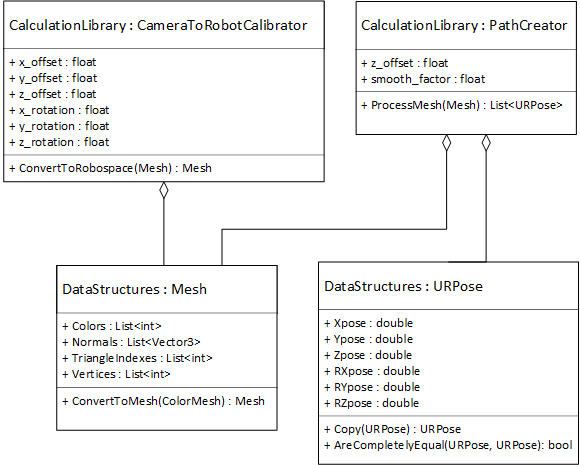
\includegraphics[width=0.7\textwidth]{figurer/d/Design/Class/uml_class_conversionlibrary}
    \caption{KLassediagram for ConversionLibrary}
    \label{class_ConversionLib}
\end{figure}
\newpage

\subsection{RoboLibrary}
Biblioteket giver mulighed for kommunikation med Robot Arm.
I det øverste modul, RoboMaster, af biblioteket vil der være mulighed for at instruere Robot Arm i at gennemløbe en mængde af positurer.

PathFeeder står for at gennemløbe hver positur i listen, og kommunikere med Data for at finde ud af hvornår den næste positur skal sendes til Robot Arm.
Data-klassen er der som en grænseflade mellem den 'logiske' del af biblioteket og dens underliggende reader/writer klasser. Reader står for kontinuerligt at læse data fra Robot Arm. Analyzer konverterer det indlæste data til en objekt-orienteret model, altså transformation af bytes til Robot Arms nuværende positur.

Writer står for at omskrive værdier til binær data. Modbus skriver binær data ud på Robot Arms IP gennem modbus-protokollen.

\begin{figure}[H]
    \centering
    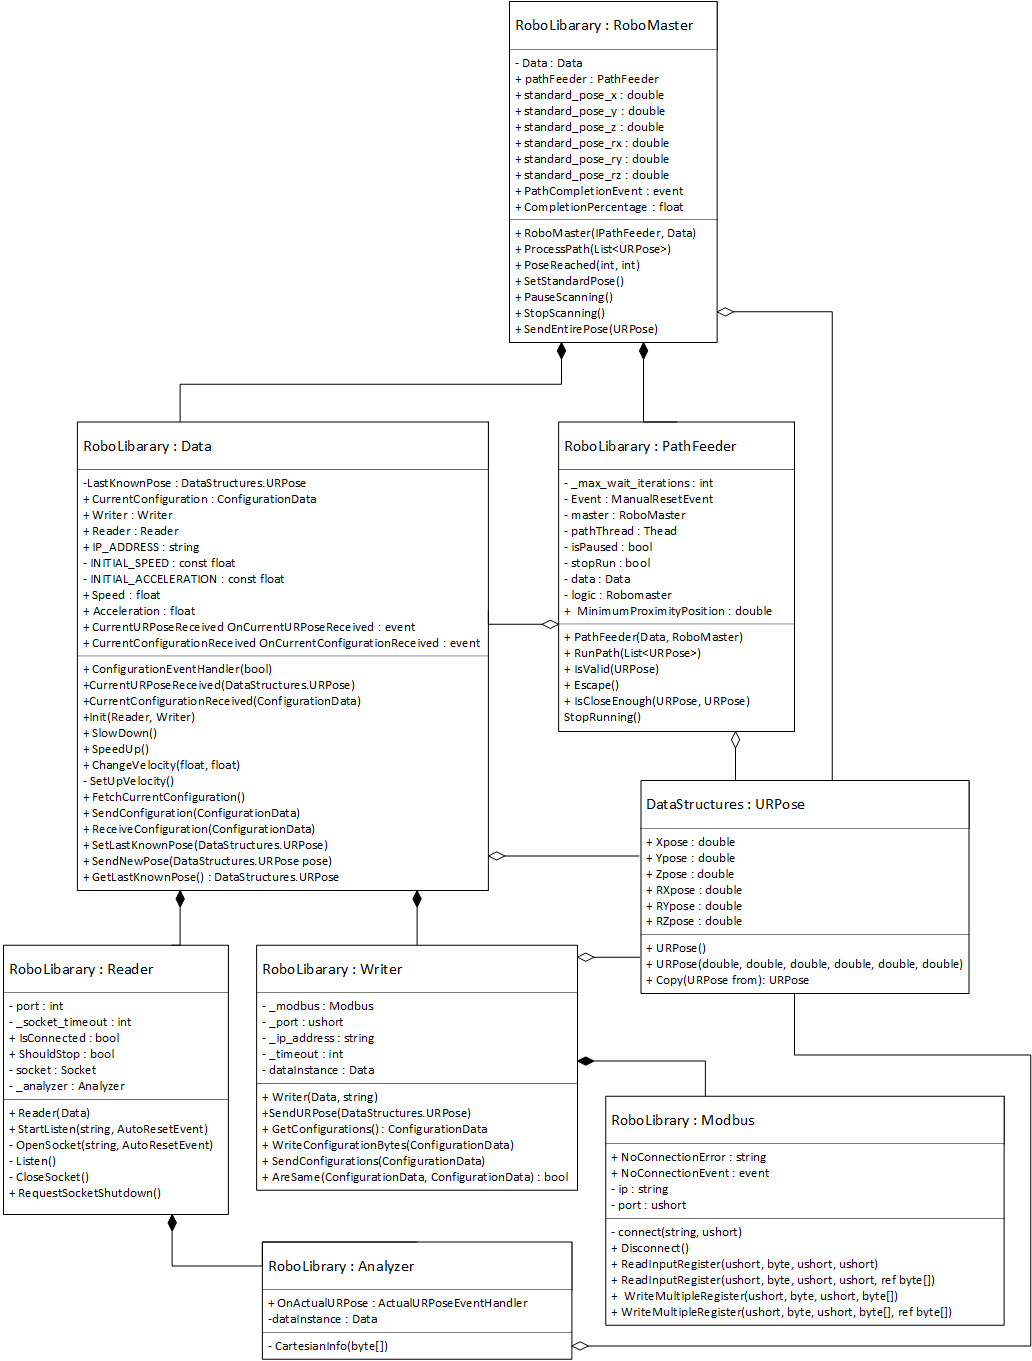
\includegraphics[width=0.75\textwidth]{figurer/d/Design/Class/uml_class_robolibrary}
    \caption{KLassediagram for RoboLibrary}
    \label{class_RoboLib}
\end{figure}





\newpage
\section{Sekvensdiagrammer}
Der er på baggrund af klassediagrammerne lavet sekvensdiagrammer, som beskriver systemets funktionalitet, og hvor de vigtigse metoder og attributter imellem klasserne er identificeret.

Nedenstående sektioner vil beskrive de vigtigste sekvensdiagrammer i system og fremvise, hvordan klasserne indbyrdes kommunikerer. 

\subsection{3D scan}
Ved scan vil KinectFusionizeren stå for at tage et dybdebillede og et farvebillede fra Kinect-sensoren.
Den vil dernæst konvertere dybdebilledet til en point cloud og give hvert punkt i skyen en farve fra farvebilledet.
Dette trianguleres, så der fås en mesh der efterfølgende kan bearbejdes. 
ComputerVisionMaster får meshen tilbage, får lavet et 2D billede af meshen fra en bestemt vinkel og giver begge tilbage GUI.
GUI viser billedet og holder på meshen indtil den skal sendes videre til ultralydsscanning

\begin{figure}[H]
    \centering
    \includegraphics[width=1\textwidth]{figurer/d/Design/Sequence/sd_3Dscan}
    \caption{Sekvensdiagram for 3D scan}
    \label{sd_3Dscan}
\end{figure}

\subsection{Feed Path}
Efter konvertering af robot space og konstateringen af stien er blevet oprettet i PathCreator skal Robot Arm instrueres i at flytte sig gennem punkterne.
PathFeeder får en liste af de positurer som den skal gennemløbe. Derefter sendes den næste i listen til Data, som videregiver posituren til Writer.
Writer konverterer posituren til binær data, og ModBus skriver dataen ud på Robot Arms register.
Hernæst ser PathFeeder på om Robot Arms nuværende positur har nærmet sig den ønskede positur. 
Når den er tæt nok på, hoppes der ud af 'while'-løkken, og den næste positur kan sendes.
Den Alt der er her skal forstås som at PathFeeder kører i sin egen baggrundstråd der kan pauses ved at sætte et flag. 
Ved terminering af denne baggrundstråd vil PathFeeder stoppe med at videregive nye positurer til Robot Arm.

\subsection{Indlæsning af Robotarms positur} 
Reader initieres med en IP hvor den skal lytte på. 
Der åbnes en socket på denne IP, og derefter lytter den kontinuert i en baggrundstråd. 
Readeren giver de rå data videre til Analyzer som konverterer dem til Robot Arms nuværende positur.

\begin{figure}[H]
    \centering
    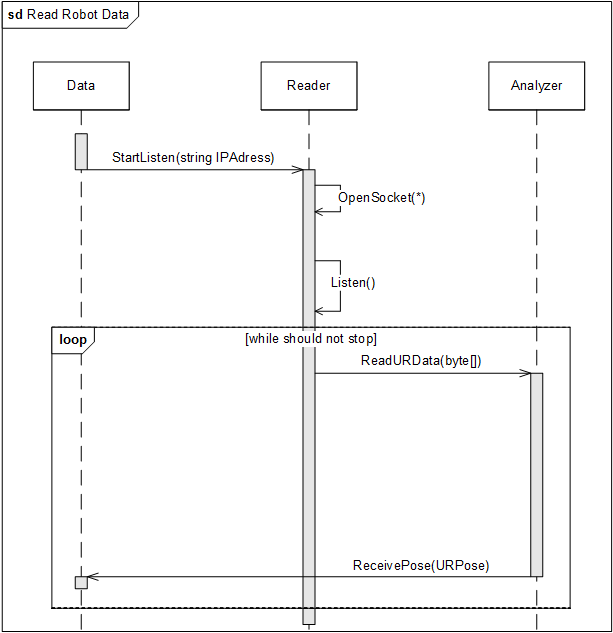
\includegraphics[width=1\textwidth]{figurer/d/Design/Sequence/sd_reading}
    \caption{Sekvensdiagram for Read Robot Data - indlæsning af Robotarms positur}
    \label{sd_reading}
\end{figure}

\subsection{Ultralydsscan}
Ved tryk på Ultralydsscan-knappen sendes den scannede mesh videre til Robomasteren (ÆNDRE PLS).
Først skal meshen konverteres fra 3D Kameras rum til Robot Arms rum, dette sker i CameraToRobotCalibrator.
Dernæst sendes den konverterede mesh til PathCreator så der oprettes en sti. 
Med denne sti får Robot Arm afdækket overfladen på Patient, hvis den har en Ultralydsscanner monteret.
Stien gives videre til PathFeeder hvor den gennemløbes. Se sekvensdiagrammet REFERENCE for forløbet her.
Når scanningen er færdig, vil GUI opdateres så Operatør ved hvornår scanningen er færdig.

\begin{figure}[H]
    \centering
    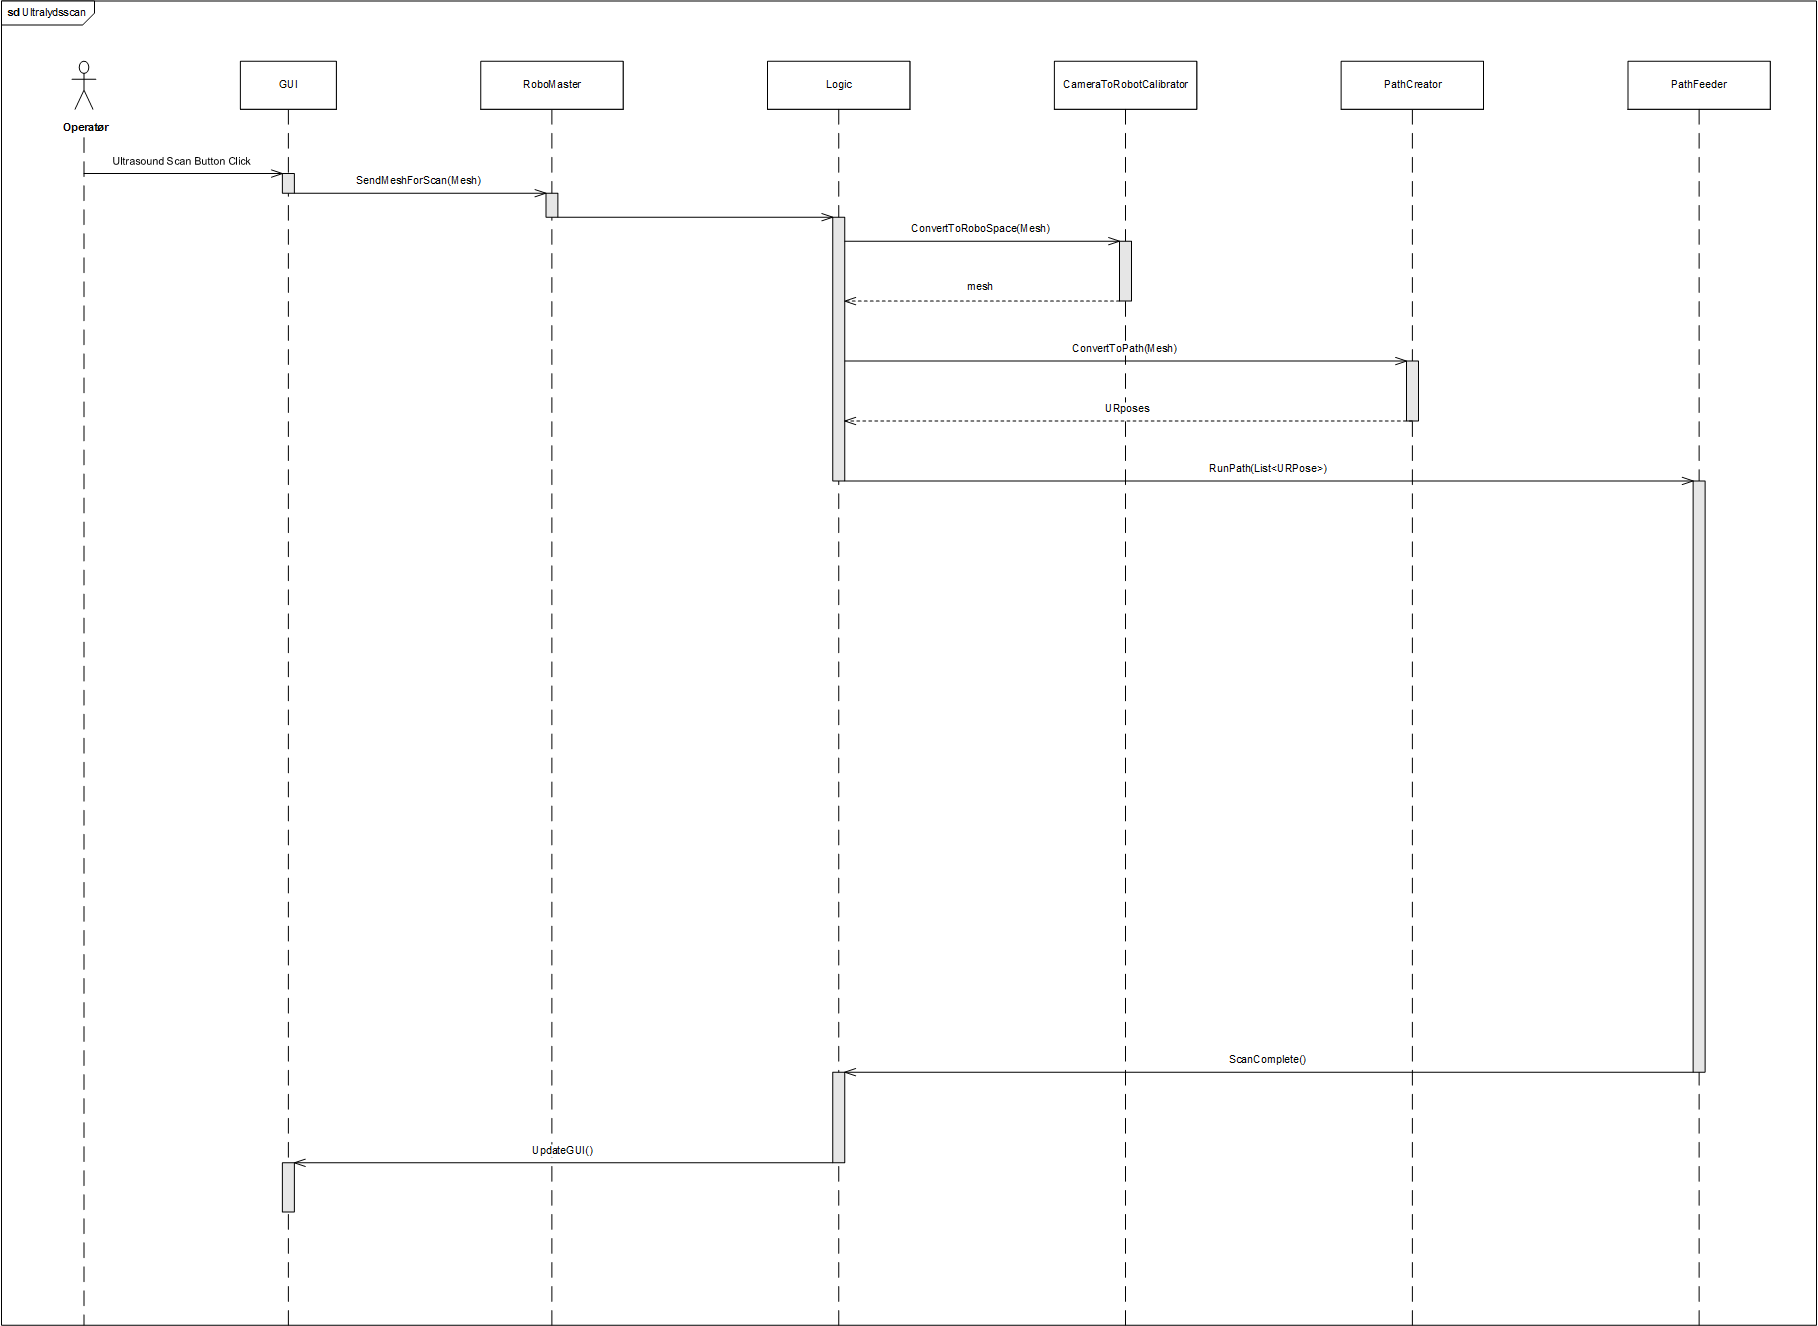
\includegraphics[width=1.2\textwidth, angle =90]{figurer/d/Design/Sequence/sd_ultrascan}
    \caption{Sekvensdiagram for Ultralydsscan}
    \label{sd_ultrascan}
\end{figure}

\section{Detajleret specifikation af klassediagrammer}
Her skal der vises metoderne i hver klasse. 

\section{Tilstandsdiagram}
Dette afsnit beskriver adfærden i systemet ved brug af et tilstandsdiagram. Tilstandsdiagrammet beskriver overgange mellem forskellige tilstande. I UC3: Ultralydsscan brystområde kan Operatør vælge at pause scanningen midlertidig og enten genoptage eller helt stoppe scanning. Figur \ref{stm_Ultra} beskriver Robotarms forskellige tilstande under udførelse af ultralydsscanning. 

\begin{figure}[H]
    \centering
    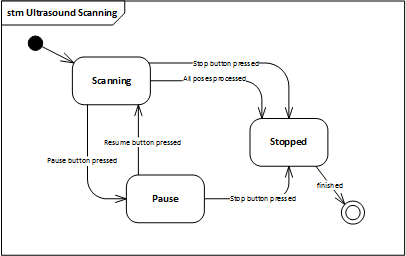
\includegraphics[width=0.7\textwidth]{figurer/d/Design/stm_UC3}
    \caption{Tilstandsdiagram for ultralydsscanning}
    \label{stm_Ultra}
\end{figure}

\section{Beregninger} 
Bare for at have det et sted og forsøge 

%% Laver piecewise funktionen 
\[ roll = \begin{cases} 
      \frac{\pi}{2}-sin^{-1}(z) & y\leq 0 \\
      \pi +cos^{-1}(-z) & y > 0 \\
   \end{cases}
\]



$$ pitch = -(\pi -atan2(y,x)) $$ Er vel det samme som   $$ pitch = atan2(y,x) - \pi $$


\[yaw = 0\] 

%%%%%%%%%%%%%%%%%%%%
% Matricerne 
\[R_M = \begin{bmatrix}
    1 & 0 & 0 \\
    0 & cos(roll) & -sin(roll) \\
    0 & sin(roll) & cos(roll)
\end{bmatrix}\] 


\[P_M = \begin{bmatrix}
    cos(pitch) & 0 & sin(pitch) \\
    0 & 1 & 0 \\
    -sin(pitch) & 0 & cos(pitch)
\end{bmatrix}\] 


\[Y_M = \begin{bmatrix}
    cos(yaw) & -sin(yaw) & 0 \\
    sin(yaw) & cos(yaw) & 0 \\
    0 & 0 & 1
\end{bmatrix}\] 

%%%%%%%%%%%%%%%%%%%%%%%%%%%% 
\[roll \geq (-\pi,\pi) \]
\[pitch \geq (-\pi,\pi) \]


\[\mathbb{R} = Y_M \cdot P_M \cdot R_M \]

%%%%%%%%%%%%%%%%%%%%%%%%
% Definerer alpha 
\[\alpha = cos^-1\bigg(\frac{\mathbb{R}_{0,0}+\mathbb{R}_{1,1}+\mathbb{R}_{2,2}-1}{2}\bigg)\] 


%%%%%%%%%%%%%%%%%%%%%% 
%Theta er lig med beregnes her 

\[ \theta = \begin{cases} 
      \alpha &  roll\geq 0 \land pitch \geq 0  \\
      2\pi-\alpha  &  roll < 0 \lor pitch < 0 \\
   \end{cases}
\]

%%%%%%%%%%%%%%%%%%%%%%% 

% mu beregnes her 
\[\mu = \frac{1}{2*sin(\theta}\]


%%%%%%%%%%%%%%%%%%%%%% 
% r_x, r_y, r_z beregnes her 

\[r_x =\mu \times(\mathbb{R}_{2,1}-\mathbb{R}_{1,2}) \times\theta \]
\[r_y =\mu \times(\mathbb{R}_{0,2}-\mathbb{R}_{2,0}) \times\theta \]
\[r_z =\mu \times(\mathbb{R}_{1,0}-\mathbb{R}_{0,1}) \times\theta \]



